\documentclass{article}
\usepackage[margin=2cm]{geometry}
\usepackage{graphicx}
\usepackage[pages=some]{background}
\usepackage{titling}
\usepackage{tabularx}
\usepackage{tikz}
\usepackage{forest}
\usepackage{float}
\usepackage{amsmath}
\usepackage{amssymb}
\usepackage{xcolor}
\usepackage{tcolorbox}
\usepackage{multicol}
\usepackage{float}

\forestset{
  my box/.style={
    draw,
    rectangle,
    rounded corners,
    fill=gray!20,
    inner sep=6pt,
    minimum width=3cm % Adjust the width as needed
  }
}


\geometry{a4paper}

\backgroundsetup{
    scale=1,
    angle=0,
    opacity=1,
    contents={%
        
\includegraphics[width=\paperwidth,height=\paperheight]{institution_logo.jpg}
    }
}

\newcommand{\subtitle}[1]{
    \posttitle{
        \par\end{center}
        \begin{center}\large#1\end{center}
        \vskip0.5em}
}

\title{ME-421}
\author{Md. Hasibul Islam}
\subtitle{FLUID MACHINERY}

\begin{document}
\begin{titlepage}
    \centering
    
    {\Huge\bfseries\maketitle}
    \textbf{Mohammad Ali Sir} \\
    \vspace{2cm}
    
\includegraphics[width=8cm]{institution_logo.jpg}
    \vfill
    \vspace*{2cm}
\end{titlepage}

\tableofcontents
\pagebreak
\section{Lecture 01: Introduction} 
\hfill Date: 03/06/2023
\subsection*{Booklist}

\textbf{Hydraulic Machines through worked out problems}

\hfill Published by BUET


\section{Lecture 2: Principles of Hydraulic Machinery}
\hfill Date: 05/06/2023

\subsection{Dynamic Action of Fluid}

When a stream of fluid enters a machine, it generally follows a specific direction. However, in order to alter its velocity, either in magnitude or direction, a force must be applied to the fluid. This force, exerted by the motion of the fluid, is referred to as dynamic force. The power of the machine is determined by the dynamic force generated by the flowing fluid, which arises due to the change in momentum.

Momentum can exist in linear or angular form, with angular momentum being the moment of linear momentum. The force is the rate of change of linear momentum, while torque is the rate of change of angular momentum. According to Newton's second law, the rate of change of momentum is proportional to the applied force and occurs in the direction of the force. Specifically, if the resultant external force in the $x$-direction is $F_x$, the mass of the fluid is $m$, the velocity of the fluid is $v_x$, and the change in velocity over time $dt$ is $dv_x$, then:
\\

The change in momentum = $mdv_x$,

And the rate of change of momentum  $= m \frac{dv_x}{dt}$
\begin{equation}
F_x = m \frac{dv_x}{dt} \label{eq:eq1}
\end{equation}

$eq^n$ (\ref{eq:eq1}) is knows as linear momentum $eq^n$.

This $eq^n$ may be wriiten as -
\begin{equation}
F_x dt = mdv_x \label{eq:eq2}
\end{equation}

This $eq^n$ is known as impulse momentum $eq^n$.

For a control volume with fluid entering in uniform velocity $v_{x_{1}}$, and leaving after time $t$ within uniform velocity $v_{x_{2}}$, then according to $eq^n$ (\ref{eq:eq2}),
\begin{equation}
	F_x = \frac{m}{t} (v_{x_{2}}-v_{x_{1}}) \label{eq:eq3}
\end{equation}

Again, $$\frac{m}{t}=\rho Q$$
\begin{equation}
	\Rightarrow F_x = \rho Q (v_{x_{2}}-v_{x_{1}}) \label{eq:eq4}
\end{equation}

Dynamic force exerted by fluid jet on stationary flat plate - 

\subsubsection{Plate normal to jet:}
A fluid jet is issued from a nozzle and strike a flat plate with a velocity $v$. The plate is held stationary at perpendicular to the centerline of the jet. Let,

\begin{center}

$Q \longrightarrow $  Volumetric flow rate\\
$\rho Q \longrightarrow$ Mass flow rate
\end{center}

Dynamic force on the fluid by the plate:
\\
Applying $eq^n$ \ref{eq:eq4}, 
$$F_x = \rho Q (v_{x_{2}} - v_{x_{1}}) $$
$$\Rightarrow -F_x = \rho Q (0-v)$$
\begin{equation}
	\Rightarrow F_x = \rho Q v \label{eq:eq5}
\end{equation}
\begin{equation}
	\Rightarrow F_x = \frac{\gamma}{g} Q v \label{eq:eq6}
\end{equation}

\begin{figure}[H]
  \centering
  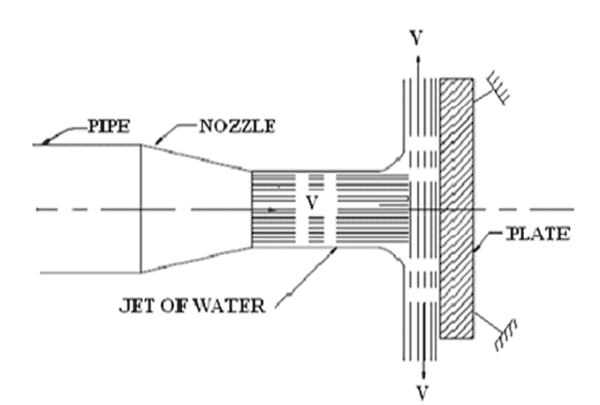
\includegraphics[width=0.75\textwidth]{img/flat_plate.png}
  \caption{Plate normal to jet.}
  \label{fig:Plate normal to jet}
\end{figure}

If $a$ is the area of jet,
$$F_x = \frac{\gamma}{g} a v  v$$
\begin{equation}
	\textcolor{red}{\Rightarrow F_x = \frac{\gamma}{g} a v^2} \label{eq:eq7}
\end{equation}

\subsubsection{Inclined Plate}
\begin{figure}[H]
  \centering
  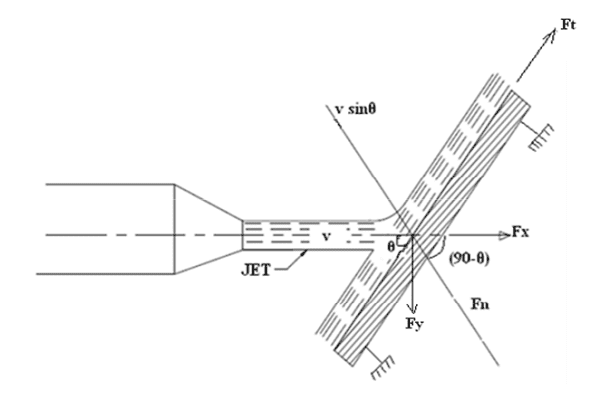
\includegraphics[width=0.75\textwidth]{img/inclined_plate.png}
  \caption{Plate inclined to jet.}
  \label{fig:Plate inclined to jet}
\end{figure}
\vspace{0.25cm}

$$F = F_n = \rho Q v sin\theta $$
Again, $$F_x = F sin\theta$$
$$= (\rho Q v sin \theta) sin \theta $$
\begin{equation}
	\textcolor{red}{F_x = \rho Q v sin^2 \theta} \label{eq:eq8}
\end{equation}
\\
And, $$F_y = F cos\theta$$
\begin{equation}
	\textcolor{red}{\Rightarrow F_y = \rho Q v sin\theta cos\theta} \label{eq:eq9}
\end{equation}
\vspace{0.25cm}
\paragraph*{Determine of division of flows:}
Let $F_s$ ($F_t$ in fig. \ref{fig:Plate inclined to jet}) be the force along the inclined surface of plate and $Q_1$ and $Q_2$ are quantities of flow along the surface. As there is no change in elevation of pressure before and after impact, the magnitude velocity leaving the plate will remain the same. \\
\\
since no force is exerted on the fluid by the plate in "S" direction, then,
\begin{equation}
	F_s = 0 = \rho Q V cos\theta \label{eq:eq10}
\end{equation}
Again, 
\begin{equation}
	\rho Q_1 v - \rho Q_2 v = 0 \label{eq:eq11}
\end{equation}

From $eq^n$ (10) \& (11),
$$\rho Q v cos\theta = \rho Q_1 v - \rho Q_2 v $$
\begin{equation}
	\Rightarrow Q cos\theta = Q_1 - Q_2 \label{eq:eq12}
\end{equation}

From continuity $eq^n$, 
\begin{equation}
	Q_1 + Q_2 = Q \label{eq:eq13}
\end{equation}

From $eq^n$ (12) \& (13),


$$Q_1 = \frac{1}{2} Q (1+cos\theta)$$ 
  \begin{equation}
     Q_2 = \frac{1}{2} Q (1-cos\theta) \label{eq:eq14} 
  \end{equation}

\pagebreak

\section{Lecture 3}
\hfill Date: 12/06/2023

\subsubsection*{Problem}
A jet of water with a velocity of 35 $m/s$ strikes a plat inclined of 30°, cross sectional area if jet 25 $cm^2$. Find the force exerted by the jet on the plate. Calculate the components of force and find the ratio in which the discharge gets divided after striking the plate. 

\subsubsection*{Solution:}
Given, 
\begin{align*}
  \text{velocity, } v &= 35 \, \text{m/s}\\
  \text{angle, } \theta &= 30^\circ \\
  \text{cross-sectional area, } a &= 25 \, \text{cm}^2 \\
  \\
  \text{Volumetric flow rate, } Q &= a \times v \\
  &= 0.0025 \times 35 \, \text{m}^3/\text{s} \\
  &= 0.0875 \, \text{m}^3/\text{s} \\ 
  \\
  \text{Force, } F &= \rho Q v \sin\theta \\
  &= 1000 \times 0.0875 \times 35 \times \sin(30^\circ) = 1531.25 \, \text{N} \\
  \\
  F_x &= F \sin\theta = 765.6 \, \text{N} \\
  F_y &= F \cos\theta = 1326.1 \, \text{N} \\
  \\
  Q_1 &= \frac{Q}{2} (1 + \cos\theta) = 0.0816 \, \text{m}^3/\text{s}\\
  Q_2 &= \frac{Q}{2} (1 - \cos\theta) = 0.00586 \, \text{m}^3/\text{s}\\
  \therefore \frac{Q_1}{Q_2} &= 13.92\\
\end{align*} 

\subsection{Thrust on moving flat plate normal to the direction of jet}
\begin{figure}[H]
  \centering
  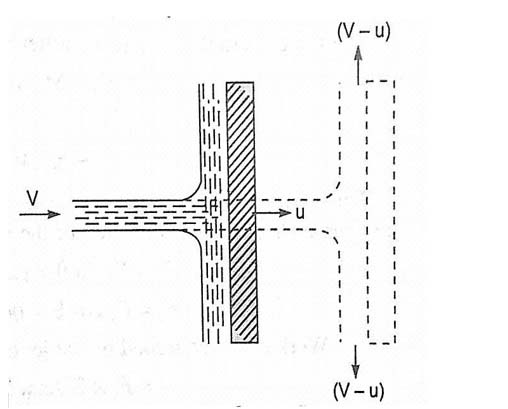
\includegraphics[width=0.5\textwidth]{img/Thrust_on_moving_flat_plate_normal_to_the_direction_of_jet.jpg}
  \caption{Thrust on moving flat plate normal to the direction of jet}
  \label{fig:Thrust_on_moving_flat_plate}
\end{figure}

Let, the flat plate moves with a velocity $u$ in the direction of the jet and the velocity of jet is $v$. The effective velocity with which the jet strike the plate = $v-u$. The mass of the fluid striking the plate per second = $\rho a (v-u)$, where $a$ is the area of the jet. \\
Thrust exerted on the plate in the direction of the jet is, 
\begin{align*}
  F &= \rho a (v-u) [(v-u) - 0]
  % F &= \rho a (v-u)^2
\end{align*}
\begin{equation}
    F = \rho a (v-u)^2 \label{eq:eq15}
\end{equation}

\begin{equation}
    \text{work done per second} = F \times u = \rho a (v-u)^{2} \times u \label{eq:eq16}
\end{equation}

However, this is not practically feasible, because the distance between the nozzle at the plate is go on increasing. If a series of plates were so arranged that each plate appeared successively before the jet in the same position and always moving with a velocity $u$ to the direction of the jet. Then mass of the fluid striking the plate = $\rho a v$.

*note : \textcolor{red}{ [ The whole flow of the nozzle is utilized by the plate. ]}

\begin{figure}[H]
  \centering
  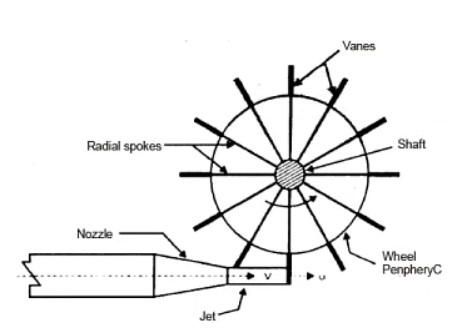
\includegraphics[width=0.5\textwidth]{img/radial_plate.jpg} 
  \caption{Thrust on Successive moving plat normal to the direction of jet}
  \label{fig:Successive_moving_plate}
\end{figure} 


The thrust on the plate,
\begin{align*}
  F &= \rho a v [(v-u) - 0] \\
  &= \rho a v (v-u)\\
\end{align*}

Work done per second = $F \times u$
\begin{equation}
  = \rho a v (v-u) u \label{eq:eq17}
\end{equation}

\begin{align*}
  \text{Now, the input power} &= \text{K.E. of the jet} \\
  &= \frac{1}{2} m v^2 \\
  &= \frac{1}{2} \rho a v \times v^2 
\end{align*}
\begin{equation}
  \therefore \text{Input power} = \frac{1}{2} \rho a v^3 \label{eq:eq18}
\end{equation}

The efficiency of the the wheel,
$$\eta = \frac{\rho a v (v-u) u}{\frac{1}{2} \rho a v^3}$$
\begin{equation}
  \eta = \frac{2u (v-u)}{v^2} \label{eq:eq19}
\end{equation}

\checkmark Generally $u$ is changed, $v$ is not changed significantly.\\

For a given jet velocity, efficiency will be maximum, if,


\begin{align*}
  \frac{d\eta}{du} &= 0 \\
  \frac{d}{du} \left[\frac{2u(v-u)}{v^2}\right] &= 0 \\
  2v - 4u &= 0 \\
  u &= \frac{v}{2}
\end{align*}

For the maximum efficiency of wheel, the peripheral speed of the wheel is equal to half of the jet velocity. \\

The max efficiency is given by - 
$$\eta_{max} = \frac{2 \frac{v}{2} (v - \frac{v}{2})}{v^2} = \frac{1}{2} = 50\% $$

\subsection{Fluid Jet (on curved plate)}
\subsubsection*{(a) stationary plate}

Velocity of jet at inlet in $x$-direction = $v_1 cos \alpha_1$ \\
Velocity of jet at outlet in $x$-direction = $v_2 cos \alpha_2$\\

Force exerted on the plate,
\begin{equation}
  F_x = \rho Q (v_1 cos \alpha_1 - v_2 cos \alpha_2) \label{ex:eq20}
\end{equation}
here, $Q = a v$   \\

If the curvature of plate at outlet such that outlet angle $\alpha_2$ is more than 90°, then the second term of the $eq^n$ (20) will be negligible. Hence in order to get more force, the curvature of the plate should be such that the angle $\alpha_2$ is obtuse.  

\subsubsection*{Single Moving Plate / Curved Vane}
\begin{figure}[H]
  \centering
  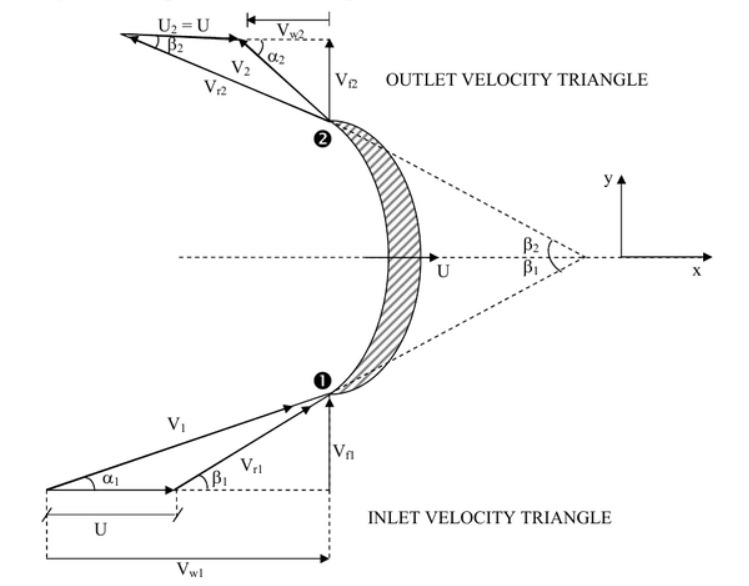
\includegraphics[width=0.8\textwidth]{img/curved_vane.jpeg} 
  \caption{Single moving plate / curved vane}
  \label{fig:curved_vane}
\end{figure} 

\begin{itemize}
  \item $v_1. v_2 \rightarrow $ Absolite velocities of the jet at inlet and outlet respectively
  \item $u_1, u_2 \rightarrow $ peripheral velocity of the vane at inlet and outlet respectively
  \item $v_{r1},v_{r2} \rightarrow $ relative velocity in inlet and outlet respectively.\\

  \begin{minipage}{0.20\textwidth}
    \begin{tcolorbox}[boxrule=1pt,width=\linewidth]
    $u + v_r = v$ \\
    $\Rightarrow v_r = v - u$ 
    \end{tcolorbox}
  \end{minipage}
  \begin{minipage}{0.33\textwidth}
    \begin{tcolorbox}[boxrule=1pt,width=\linewidth]
    $v_w, v_f$ is the components of $v$
    \end{tcolorbox}
  \end{minipage}

  \item $v_{f1}, v_{f2} \rightarrow $ velocity of flow at inlet and outlet respectively. alternatively, components of absolute velocity normal to the direction of motion.
  \item $v_{w1}, v_{w2} \rightarrow $ velocity of whirl at the inlet and outlet respectively. alternatively, components of absolute velocity in the direction of motion.  
\end{itemize}

\section{Lecture 4: Curved Vane}
\hfill Date: 17/06/2023

\subsection{Analysis of Curved Vane}
The jet enters the vane without shock if the relative $v_{r_1}$ makes an angle $\beta_1$ with the direction of motion (on x-axis). The jet glides over the vane and leaves with a velocity $v_{r_2}$. If the vane is smooth, then $v_{r_1} = v_{r_2}$. the jet will leave the vane without shock if the relative velocity $v_{r_1}$ makes an angle in $\beta_2$. \\

The mass flow rate of fluid = $\rho Q = \rho a v_r$ , where a $\rightarrow$ area of jet. 

\begin{itemize}
  \item Note: if there is only single vane, then relative velocity $v_r$ have to consider, otherwise total velocity $v$ will be counted. 
\end{itemize}

Force on the vane in the direction of motion , if $\alpha_2  < 90$°,
$$F_x = \rho a v_{r_1} \left[v_{w_1} - \left(-v_{w_2}\right)\right]$$
\begin{equation}
  F_x = \rho a v_{r_1} \left(v_{w_1} + v_{w_2}\right) \label{eq:eq21}
\end{equation}
if $\alpha_2  > 90$°, 
\begin{equation}
  F_x = \rho a v_{r_1} \left(v_{w_1} - v_{w_2}\right) \label{eq:eq22}
\end{equation}

if $\alpha_2  = 90$°, 
\begin{equation}
  F_x = \rho a v_{r_1} \left(v_{w_1} \right) \label{eq:eq23}
\end{equation}

This is the general expression of the thrust - 
$$F_x = \rho a v_{r_1} \left[v_{w_1} \pm  v_{w_2}\right]$$

if $u_1=u_2=u$, work done per second = $F_x \times u$
\begin{equation}
  = \rho a v_{r_1} \left[v_{w_1} \pm  v_{w_2}\right] \times u  \label{eq:eq24}
\end{equation}

Also work done can be determined for the changing kinetic energy. Thus the work done per second
\begin{equation}
  \text{Thus the work done per second} = \frac{1}{2} \rho a v_{r_1} \left[v_1^2 - v_2^2\right]  \label{eq:eq25}
\end{equation}

From the equation (24) \& (25),
\begin{equation}
  2(v_{w_1} \pm v_{w_2}) u = v_1^2 - v_2^2 \label{eq:eq26}
\end{equation}

Input energy of jet at inlet = $\frac{1}{2} \rho a v_1 \times v_1^2 $

The hydraulic efficiency, $$\eta = \frac{\rho a v_{r_1}  \left[v_{w_1} \pm  v_{w_2}\right] u}{\frac{1}{2} \rho a v_1 \times v_1^2}$$
\begin{equation}
  \eta = \frac{2 u v_{r_1}  \left[v_{w_1} \pm  v_{w_2}\right]}{v_1^3}  \label{eq:eq27}
\end{equation}
\pagebreak

\section{Lecture 5: Series of Vanes}
\hfill Date: 19/06/2023

If a series of vanes is fixed radially to the rim of a wheel, there is always one vane or another facing the jet. Thus the entire fluid is utilized. This arrangement of vanes is used in radial flow turbines.\\

Two types of radial flow turbine: 
\begin{enumerate}
  \item Inward flow turbine : If jet enters outer periphery
  \item Outward flow turbine : If jet enters inner periphery
\end{enumerate}

Let $R_1$ and $R_2$ be the radii of the wheel at the inlet and outlet.

\begin{figure}[h]
  \begin{center}
  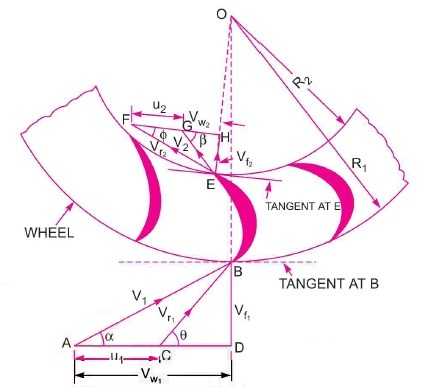
\includegraphics[width=0.8\linewidth]{img/series_vane.jpg}
    \caption{Series of vanes}
\end{center}
\end{figure}

Let, $\omega$ is the angular velocity of the wheel,
$$u_1 = \omega R_1 = \frac{2 \pi N}{60} R_1$$
$$u_2 = \omega R_2 = \frac{2 \pi N}{60} R_2$$
here, N = RPM \\
Let $m$ be the mass flow rate striking the vane. The momentum in the tangential direction at the inlet = $mv_w$ \\
The moment of momentum about the center at inlet = $mv_{w_1}R_1$\\
The moment of momentum about the center at outlet = $-mv_{w_2}R_2$\\
$\therefore$ Torque on the wheel,
$$T = mv_{w_1}R_1 - \left(-mv_{w_2}R_2\right)$$
\begin{equation}
  T = m \left(v_{w_1}R_1 + v_{w_2}R_2\right) \label{eq:eq28}
\end{equation}

\begin{align*}
  \text{Work done per second} &= T \times \omega \\
  &= m \left(v_{w_1}R_1 + v_{w_2}R_2\right) \times \omega \\ 
\end{align*}
\begin{equation}
  \text{work done per second} = m \left(v_{w_1}u_1 + v_{w_2}u_2\right)  \label{eq:eq29}
\end{equation}
Here, $\beta<$  90° \\


If $\beta>$  90°,  
\begin{equation}
  \text{work done per second} = m \left(v_{w_1}u_1 - v_{w_2}u_2\right)  \label{eq:eq30}
\end{equation}

The general expression,  
\begin{equation}
  \text{work done per second} = m \left(v_{w_1}u_1 \pm v_{w_2}u_2\right)  \label{eq:eq31}
\end{equation}
\text{This equation is known as Euler Pump Turbine equation.}

Hydraulic Efficiency,
\begin{equation}
  \eta_h = \frac{m\left(v_{w_1} u_1 \pm v_{w_2} u_2\right)}{\frac{1}{2} m v_1^2} = \frac{2\left(v_{w_1} u_1 \pm v_{w_2} u_2\right)}{v_1^2}
  \label{eq:eq32}
\end{equation}

\subsubsection*{Problem 01}
A jet of water having a velocity of 30 $ms^{-1}$ impinging for a series of vanes mounted on the periphery of a wheel moving with a peripheral velocity of 15 $ms^{-1}$. The aboslute velocity is directed at an angle of 30° to the direction of motion of vanes. The relative velocity at outlet is 95\% of the value at inlet. The absolute velocity at exit is normal to the direction of the motion of the vane. Assuming smooth entry, find the vanes angle at inlet and outlet and the hydraulic efficiency of vane. \\
\textbf{Solution}: 

\begin{multicols}{2}
  given, \\
  $v_1$ = 30 m/s \\
  $\alpha$ = 30° \\
  $u_1$ = 15 m/s \\
  $v_{r_2} = 0.95 \times v_{r_1}$ \\
  $\beta$ = 90° [normal] \\
  so, $v_{w_2} = 0, v_{2} = v_{f_2}$ \\ 
  $\checkmark$ have to add figure in exam 
\end{multicols}

\begin{multicols}{3}
  \begin{align*}
    v_{w_1} &= v_1 \cos 30 \\
    &= 30 \cos 30 \\ 
    &= 25.98 \, m/s   
  \end{align*}

  \begin{align*}
    \tan \theta &= \frac{v_{f_1}}{v_{w_1} - u_1}\\
    \theta &= 53.8    
  \end{align*}

  \begin{align*}
    v_{r_1} &= \sqrt{\left[v_{w_1} - u_1\right]^2 + (v_{f_1})^2}\\
    &= 18.59 \, m/s   
  \end{align*}

  \begin{align*}
    v_{r_2} &= 0.95 \times v_{r_1}\\
    &= 17.67 \, m/s   
  \end{align*}

  \begin{align*}
    & \text{Assuminng } u_1 = u_2, \\
    \cos \phi &= \frac{v_{f_2}}{u_2}\\
    \phi &= \cos^{-1} \left(\frac{15}{17.66}\right) \\ 
    &= 27.53 
  \end{align*}

  \begin{align*}
    \eta_h &= \frac{2 v_{w_1} u_1}{v_1^2}\\
    \eta_h &= \frac{2 \times 25.98 \times 15}{30^2}\\
    &= 0.866 \\
    &= 86.7\%  
  \end{align*}


\end{multicols}

\subsubsection*{Problem 02}
A jet of water 5 cm in diameter inpinges on a curved vane and is deflected through an angle of 175°. The vane moves in the same direction at that of the jet with a velocity of 35 m/s. The rate of flow is 170 l/s. Determine the compounds forces, horse power developed by the vane and water efficiency. Neglect friction. Solve this problem, if instead of one vane, there are a series of vanes fixed to a wheel.\\
$F_x = ?, F_y = ? , HP = ?, \eta_h = ?$\\

\textbf{Solution:} 
\begin{multicols}{2}
  Given,\\
  d = 5 cm \\
  u = 35 m/s \\
  Q = 170 l/s = 0.17 $m^3/s$ \\
  $$v = \frac{Q}{a} = \frac{0.17}{0.196\times 10^{-2}} = 86.58 /, m/s$$ \\
  $$a = \frac{\pi}{4} \left[0.05\right]^2 = 0.196 \times 10^{-2} /, m^2$$ \\
  v= u + $v_r$ \\
  $v_r = 86.58 - 35 = 51.58$ m/s \\ 
\end{multicols}

Neglecting friction,\\
\begin{align*}
  v_{r_1} = v_r &= 51.58 \, m/s \\\
  v_{r_1} \cos \phi &= 51.38 \, m/s \\
  \therefore v_{w_1} = v_{r_1} \cos \phi - u_1 &= 51.38 -35 = 16.38 \, m/s \, [u = u_1] \\ 
\end{align*}

\begin{align*}
  F_x &=\rho a v_r \left(v_w + v_{w_1}\right) = 10427.87 N \\
  F_y &=\rho a v_r \times v_{f_1} \\
  HP &= \frac{F_x u}{746} \\
  \eta_h &= \frac{F_x u}{\frac{1}{2} m v^2} =  \frac{10427.87 \times 35}{\frac{1}{2} \times 1000 \times 0.17 \times 86.58^2} = 57.3\% 
\end{align*}
\hrulefill


\section{Lecture 6: Hydraulic Turbines}
\hfill Date: 24/06/2023

Hydraulic turbines are the machines which converts the hydraulic energy into mechanical energy. In other words, hydraulic turbines are prime movers which run with hydraulic energy. The mechanical energy produced by a hydraulic turbine can be connected into electric energy by coupling the turbine to an electric generator. 

\subsection*{Classfications of Turbines}
May be classified according to the following criteria:
\begin{enumerate}
  \item Hydraulic action 
  \item Direction of fuel of water 
  \item Direction of the shaft
  \item Head 
  \item Specific Speed 
\end{enumerate}

\subsubsection*{Prime Mover}
Prime movers refer to the mechanical devices or systems that convert hydraulic energy (the energy of flowing or falling water) into mechanical energy (rotational motion). These prime movers are responsible for driving the turbine rotor and generating power. In the case of hydraulic turbines, the most common type of prime mover is an electric generator or alternator. The turbine is connected to the rotor of the generator, and as the turbine rotates, it transfers its mechanical energy to the generator, which then converts it into electrical energy. The prime mover can also be a mechanical drive system, such as a gearbox or a shaft, which is connected to various industrial machines or equipment. In such cases, the mechanical energy produced by the turbine is directly transmitted to the driven machinery to perform specific tasks. The choice of prime mover depends on the application and the desired output. In most large-scale hydropower plants, electric generators are used as prime movers to produce electrical power that can be transmitted over long distances and distributed to consumers. In other industrial applications, mechanical prime movers may be employed for specific operations within a facility.

\subsubsection*{Specific Speed}
The specific speed of a hydraulic turbine is a dimensionless parameter that characterizes the geometric and hydraulic performance of the turbine. Specific speed (Ns) is defined as the speed at which a geometrically similar turbine would operate to produce unit power (1 horsepower or 1 kilowatt) under a unit head (1 foot or 1 meter).

\subsection*{Hydraulic Action}
\begin{enumerate}
  \item \textbf{Impulse Turbine:} Here the available head is converted into kinetic energy by passing the water through a nozzles. Ex - Pelton wheel, girard turbine, banki turbine etc. 
  \item \textbf{Reaction Turbine:} A part of the total head is connected in kinetic energy and the rest remains in the form of pressure energy. Example of reaction turbines - kaplan turbine, propeller turbine, etc. 

\end{enumerate}

\subsection*{Direction of flow of water}
\begin{enumerate}
  \item Tangent flow turbine : The water strikes the runner in the direction of tangent to the wheel. Ex - pelton wheel. 
  \item radial flow turbine: may be classified as inward flow and outward flow. Ex - francis turbine (old) (inward flow)
  \item Axial Flow : Kaplan and propeller turbine 
  \item Mixed Flow Turbine : Francis turbine 
\end{enumerate}

\subsection*{Direction of the shaft}
\begin{enumerate}
  \item Vertical : shaft vertical, runner horizontal 
  \item Horizontal : shaft horizontal, runner vertical 
\end{enumerate}

\subsection*{Head}
\begin{enumerate}
  \item High Speed Turbine: Net head is 150m - 2000 m. Ex - pelton wheel turbine 
  \item Medium Head Turbine: Head from 30 m - 150 m. Ex - Francis Turbine 
  \item Tow Head Turbine: Head < 30 m. Ex - Kaplan and propeller. (kaptai)  
\end{enumerate}

\subsection*{Specific speed}
\begin{enumerate}
  \item Low Specific Speed : speed < 60. Ex - pelton wheel 
  \item Medium Specific Speed : 60 < speed < 400.  Ex - Francis turbine. 
  \item High Specific Speed: speed > 400. Ex - Kaplan Turbine. 
\end{enumerate}

\subsection*{Difference between axial and radial hydraulic turbine }
\begin{itemize}
  \item Fluid Flow Direction:

  \textbf{Axial Hydraulic Turbine}: In an axial hydraulic turbine, the water flow is parallel to the axis of rotation. The water enters the turbine axially and passes through the rotor blades in the same axial direction.\\

  \textbf{Radial Hydraulic Turbine}: In a radial hydraulic turbine, the water flow is radial, moving inward or outward from the center of the turbine. The water enters the turbine radially and flows through the rotor blades in a radial direction.
  \item Blade Orientation and Configuration:
  
  \textbf{Axial Hydraulic Turbine}: Axial turbines have rotor blades arranged in a propeller-like configuration, similar to the blades of a ship's propeller. The blades are oriented parallel to the axis of rotation and typically have a streamlined shape to efficiently capture the water's energy.\\

  \textbf{Radial Hydraulic Turbine}: Radial turbines have rotor blades arranged in a radial pattern, perpendicular to the axis of rotation. The blades extend radially from the center of the turbine and are typically straight or slightly curved. They are designed to effectively capture the water flow in a radial direction.
  \item Applications:
  
   \textbf{Axial Hydraulic Turbine}: Axial turbines are commonly used in high-flow, low-head applications, such as in large-scale hydropower plants. They are suitable for situations where a large volume of water needs to be harnessed efficiently.\\

  \textbf{Radial Hydraulic Turbine}: Radial turbines are typically employed in low-flow, high-head applications. They are often used in small-scale hydropower installations, such as run-of-river projects or micro-hydropower systems.

  \item Efficiency and Performance:
  
  \textbf{Axial Hydraulic Turbine}: Axial turbines are known for their high efficiency at high flow rates. They can handle a significant volume of water and are well-suited for sites with a substantial water supply.\\

  \textbf{Radial Hydraulic Turbine}: Radial turbines are efficient in applications where there is a significant pressure drop. They are designed to generate power under high head conditions, where water is available at a relatively low flow rate.
\end{itemize}
\hrule

\section{Lecture 7: Pelton Wheel}
\hfill Date: 08/07/2023

Mainly 2 types of turbine:
\begin{enumerate}
  \item Impulse Turbine 
  \item Reaction Turbine 
\end{enumerate}

\checkmark  Force always acts perpendicular to the wall. 
\subsection*{Pelton Wheel}
The whole hydraulic energy is converted into kinetic energy. 

\subsection*{Major Components}
\subsubsection*{a) Nozzle With Control Mechanism}
The jet velocity remains the same and only the discharge changes. 
\subsubsection*{b) Buckets \& Runner}
A pelton wheel is fitted with buckets havingthe shape of double hemispherical cup. The angle at the outlet teeth varies from 10° to 20° and the jet deflects 170°-160°.\\

The advantage of double cup bucket is that because of symmetric, the axial thrust on the shaft is zero. 

\begin{figure}[h]
  \begin{center}
    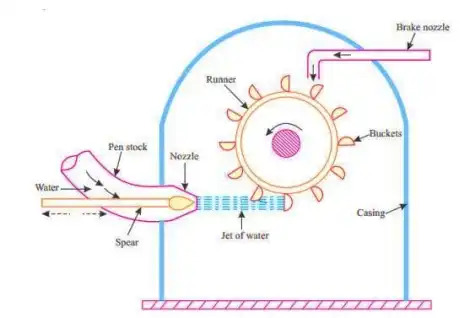
\includegraphics[width=0.8\linewidth]{img/PELTON-TURBINE.png}
    \caption[Pelton wheel components]{Pelton wheel components}
  \end{center}
\end{figure}

\subsubsection*{Casing}
\begin{itemize}
  \item To prevent splashing 
  \item To lead the water to tail race 
  \item To act as a safeguard against accident 
\end{itemize}

\subsubsection*{Hydraulic Brake}
The hydraulic brake consists of a small nozzle which directs a jet on the back of the bucket, in the opposite direction which causes braking.

\subsubsection*{Deflector}
The sudden closing of the nozzle may cause excessive water hammer. To avoid water hammer, the nozzle is closed slowly by a moveable steel plate known as deflector. 


\subsubsection*{Why Pelton wheel deflection angle is not set for 180°}
Although, deflection angle 180° will give the best thrust, it is not set in pelton wheel. When water flows through the Pelton wheel, it strikes the buckets or cups, causing the wheel to rotate. The design of the buckets is crucial for efficient energy transfer. The water jet enters the bucket at a specific angle, known as the jet's deflection angle.

If the deflection angle were set to 180 degrees, the water jet would hit the bucket and then reverse its direction completely, flowing back in the opposite direction. This would result in a loss of kinetic energy and disrupt the smooth operation of the wheel.

To maximize the energy transfer, the deflection angle is typically set to less than 180 degrees. Ideally, the water jet should leave the bucket with minimal residual velocity, meaning that most of its kinetic energy has been transferred to the wheel. This is achieved by setting the deflection angle at a value that allows the water jet to leave the bucket at an optimal angle, usually around 160 to 170 degrees.


\subsection*{Expression of work done}
Effective head, H = Gross head - $h_f$ \\
$h_f \rightarrow$ loss of head in the penstock\\ 

torque,
$$T = \rho a v \left[v_w R - (v_{w1} R_1)\right] = \rho a v \left(v_w R + v_{w1}R_1 \right)$$

$$W = T \times \omega = \rho a v \left(v_w R + v_{w1} R_1\right) \times \omega $$

Now, $R \omega = u, R_1 \omega_1 = u_1$
$$W = \rho a v \left(v_w u + v_{w1} u_1\right) $$

In general,
\begin{equation}
  W = \rho a v \left(v_w u \pm v_{w1} u_1\right) \label{eq:eq33}
\end{equation}

\begin{figure*}[h]
  \begin{center}
    \includegraphics*[width=0.8\linewidth]{img/pelton_force.jpeg}
    \caption{Force analysis on pelton wheel}
  \end{center}
\end{figure*}

Let, $u=u_1$
\begin{align*}
  W &= \rho a v \left(v_w + v_{w1} \right) \times u \\
  &= \rho a v \left(v + v_{r1} \cos \phi - u \right) \times u \\
  &= \rho a v \left(v - u + K v_{r} \cos \phi \right) \times u \\
  &= \rho a v \left[(v - u) + K (v-u) \cos \phi \right] \times u \\
  &= \rho a v (v - u)(1 + K  \cos \phi)  \times u 
\end{align*}

\begin{equation}
  W = \rho a v (v - u)(1 + K  \cos \phi)  \times u \label{eq:eq34}
\end{equation}

Neglecting losses in nozzle,\\
 \begin{equation}
 \text{Input power} = \frac{1}{2} \rho a v \times v^2 \label{eq:eq35}
\end{equation}

Hydraulic efficiency,
\begin{align*}
  \eta_h &= \frac{\text{work done}}{\text{input power}} \\ 
  &= \frac{\rho a v (v - u)(1 + K  \cos \phi)  \times u}{\frac{1}{2} \rho a v \times v^2}
\end{align*}
\begin{equation}
  \eta_h = \frac{ 2 (v - u)(1 + K  \cos \phi)  \times u}{v^2} \label{eq:eq36}
 \end{equation}

 \vspace*{1cm}

 \section{Lecture 8: Working proportions of Pelton Wheel}
\hfill Date: 10/07/2023

$\eta_h$ will be maximum if, 
\begin{align*}
  \dfrac{d\eta_h}{du} &= 0 \\
  \frac{d}{du} \left\{2 (v-u) (1 + K \cos \phi) u \right\} &= 0 \\
  v - 2u &= 0 \\
  u &= \frac{v}{2}
\end{align*}

now, 
\begin{align*}
  (\eta_h)_{max} &= \frac{ 2 (v - \frac{v}{2})(1 + K  \cos \phi)  \times \frac{v}{2}}{v^2} \\
  &= \frac{ \frac{v^2}{2}(1 + K  \cos \phi)}{v^2} \\
  &= \frac{1 + K  \cos \phi}{2}
\end{align*}

If K=1, i.e. the vanes are smooth,
$$\eta_h = \frac{1 + \cos \phi}{2}$$
The $\eta_h$ is less than unity, because K is always less than unity and $\phi \neq  0$
\\

The work done by a pelton wheel may also be expressed as the difference of kinetic energy at the inlet and outlet. This work done = $\frac{1}{2} \rho a v \left(v^2 - v_1^2\right)$

\begin{equation}
  \eta_h = \frac{\frac{1}{2} \rho a v \left(v^2-v_1^2\right)}{\frac{1}{2} \rho a v v^2} = \frac{v^2-v_1^2}{v^2} \label{eq:eq37}
\end{equation}

The mechanical efficiency $(\eta_m)$ is defined as the ratio of the power obtained at the shaft (S.P.) to the power developed by the runner. Thus,
\begin{equation}
  \eta_m = \frac{S.P.}{P} \label{eq:eq38} 
\end{equation}

The overall efficiency, 
\begin{equation}
  \eta_o = \frac{S.P}{\text{Power supplied ti the turbine} (P_t)} = \frac{S.P}{P} \times \frac{P}{P_t} = \eta_h \times \eta_m \label{eq:eq39}
\end{equation}

\subsection*{The working proportions of pelton wheel}
\begin{enumerate}
  \item Velocity of Jet: 
  $$V_{theo.} = \sqrt{2g H}$$ Here, H = net head. Now actual velocity,
  \begin{equation}
    V = C_v \sqrt{2g H}  
    \label{eq:eq40}
  \end{equation}
$$C_v = 0.97 \sim  0.99$$

\item Theoretical Power ($P_t$)
\begin{equation}
  P_t = \gamma Q H
  \label{eq:eq41}
\end{equation}

\begin{center}
\begin{minipage}{0.5\textwidth}
    \setlength{\fboxrule}{1pt} % Border thickness
    \setlength{\fboxsep}{10pt} % Padding
    \fbox{%
        \parbox{\dimexpr\linewidth-2\fboxsep-2\fboxrule}{%
            $\frac{1}{2} m v^2 = \frac{1}{2} m \times 2g H = m g H = \rho Q g H = \gamma Q H $
        }%
    }
  \end{minipage}
\end{center}

\item Angle ($\theta$)

The angle varies from 10°-20°. The average value of angle is 15°. 

\item Diameter of Jet($\alpha$)

The diameter of jet may be obtained if the discharge is low. 
$$\frac{\pi}{4} d^2 = \frac{Q}{C_v \sqrt{2gH}}$$
\begin{equation}
  d = \left(\frac{4Q}{\pi C_v \sqrt{2gH}}\right)^{\frac{1}{2}}
\end{equation}

\item Speed Ratio ($K_u$)

It is the ratio of the velocity of the wheel at pitch circle (u) to the theoretical velocity of the jet,
\begin{equation}
  K_u = \frac{u}{\sqrt{2gH}} \label{eq:eq43}
\end{equation}
$K_u$ varies from $0.43 \sim 0.47$ 

\item Mean diameter of the wheel (D)

The diameter of the wheel measured upto the center of the bucket is called the mean diameter. 
$$u = \frac{\pi D N}{60}$$

\begin{equation}
  D = \frac{60 u}{\pi N}
\end{equation}
D is also known as pitch diameter. 

\item Jet Ratio ($J_r$)
\begin{equation}
  J_r = \frac{D}{d} 
\end{equation}

$J_r$ varies from 11 to 14. 

\item Size of Bucket 

The flowing proportion of the bucket are usually adopted. \\
Radial length of the bucket = $(2 \sim 3) \times d $\\
Axial width of the bucket = $(3 \sim 5) \times d $ \\
Depth of the bucket = $(0.8 \sim 1.2) \times d $ \\
Where, 'd' is the diameter of the jet. 

\item Number of Jets

Ordinarily pelton wheel has a single jet, but to develop more power, it has number of jets. More than 6 jets are not provided. 

\item Number of Buckets (z)

Number of buckets should be as small as possible. So as to keep the frictional losses to a minimum. But number of buckets should also be sufficiently large, so that the jet is always intercepted by one bucket or another. The jet will always be intercepted by the buckets if the angle between two successive buckets is equal to or less than $2\theta$, such that $$\cos \theta = \frac{R+\frac{d}{2}}{r_o}$$
or, $$\sin \theta = \sqrt{1 - \cos^2 \theta} = \left[1- \left(\frac{R + \frac{d}{2}}{r_o}\right)^2\right]^{1/2} $$

\begin{figure*}[H]
  \begin{center}
    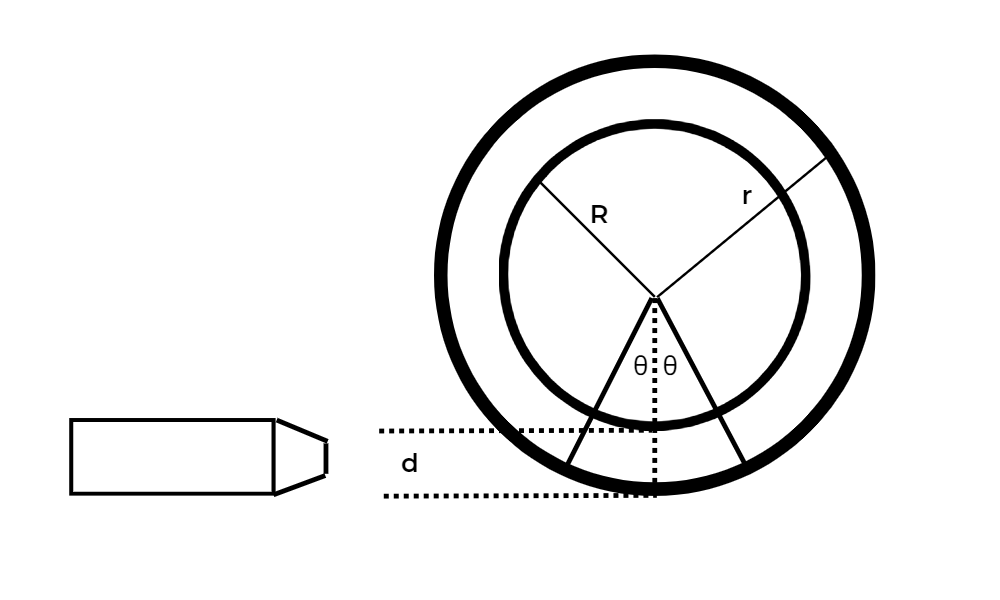
\includegraphics[width=0.9\linewidth]{img/number_of_bucket.png}
    \caption{Parameters for Pelton wheel}
  \end{center}
\end{figure*} 

For a small $\theta$, $\sin \theta \approx \theta $
$$\theta = \left[1- \left(\frac{R + \frac{d}{2}}{r_o}\right)^2\right]^{1/2} $$

Therefore, the number of buckets is given by, $$z = \frac{2\pi}{2\theta} = \frac{\pi}{\theta}$$
\begin{equation}
  z = \frac{\pi}{\left[1- \left(\frac{R + \frac{d}{2}}{r_o}\right)^2\right]^{1/2}}
\end{equation}

Emperical formula given by Taygun,
$$z = \frac{D}{2d} + 15$$
\begin{equation}
  z = 0.5 J_r + 15  
\end{equation}
Here, $J_r = $ Jet Ratio 
\end{enumerate}

\vspace*{1cm}
\pagebreak
\section{Lecture 9: Problems on Pelton Wheel}
\hfill Date: 17/07/2023

\begin{multicols*}{2}
  \subsubsection*{Problem-01}
  A single jet pelton turbine is required to drive a generator to develop 10000 kw. The available head at the nozzle is 760m. Assuming electric generator efficiency as 95\%, pelton wheel efficiency 87\%, coefficient of velocity for nozzle as 0.97, mean bucket velocity as 0.46 of jet velocity. Outlet angle of the bucket as 15° and the relative velocity of water leaving the bucket as 0.85 of that at inlet. Find: a) Diameter of jet, b) The flow in cumecs, c) The force exerted by the jet on the bucket, d) If the ratio of mean bucket circle diameter to the jet diameter is not to be less than 10, find the synchronous speed for generator at 50 cycles/second and the corresponding mean diameter of the runner.

  \subsubsection*{Solution:}
  Given, P = 10000 kW, H = 760 m, $\eta_g = 0.95, \eta_h = 0.85, C_v = 0.97$, u = 0.46 v, $\phi = 15\deg , V_{r1} = 0.85 V_r$, f=50 hz, $\frac{D}{d} > 10 $ \\

  Available power at the wheel = $\frac{10000}{0.95} = 10526.3$ kW \\
  Now, \begin{align*}
    \eta_h &= \frac{10526.3\times 10^3}{\gamma Q H} \\
    0.87 &= \frac{10526.3\times 10^3}{9810 \times Q \times 760} \\
    Q &= 1.623 \, cumecs 
  \end{align*}
  Again,
  \begin{align*}
    Q &= \frac{\pi}{4} d^3 \times C_v \times \sqrt{2gH} \\
    d &= 0.132 \, m 
  \end{align*}
  Assuming $D/d=10$, D = 1.32 m \\
  Now, $$v_w = v = 0.97 \times \sqrt{2\times 9.81\times 760} = 118.5 \, m/s$$
  $$u = 0.46 \times v = 54.51 \, m/s$$ 
  $$v_r = v_w - u = 64 \, m/s$$
  $$v_{r1} = 0.85 v_r = 54.4 \, m/s$$ 
  $$v_{w1} = v_{r1} - v_{r1} \cos \phi = 544 -52.55 = 2 \, m/s $$
  $$\text{Force} = \rho Q (v_w - v_{w1}) = 1000 \times 1.623 \times (118.5-2)$$ So, Force = 189.1 \, kN 

  Again, \begin{align*}
    u &= \frac{\pi D N}{60} \\
    N &= 788 \, rpm 
  \end{align*}

  Now, \begin{align*}
    N &= \frac{120 \times f}{Pole}\\
    Pole &= 7.614 \approx 8
  \end{align*}

  Putting, Pole = 8, $N = \frac{120f}{8} = 750 rpm$\\
  $$u=\frac{\pi D\times 750}{60} \Rightarrow D = 1.388 \, m$$
  \vspace*{0.5cm} 

  \subsubsection*{Problem-02}
  A pelton wheel is developing 11000 kW under a head of 650 m at 600 rpm. The peripheral velocity of wheel is 0.47 times the jet. The coefficient of velocity is 0.97 and overall efficiency is 85\%. Find jet diameter, wheel diameter, and number of buckets. 

  \subsubsection*{Solution:} 
  P = 11000 kW, H = 650 m, N = 600 rpm, $C_v = 0.97, \eta_o = 0.85$

  \begin{align*}
    &\eta_o = \frac{P}{\gamma Q H} \\
    & Q = 2.03 \, m^3/s  
  \end{align*}
  again, \begin{align*}
    &Q = \frac{\pi}{4} d^2 \times v \\
    & d = 0.1528 \, m  
  \end{align*}

  $$V = C_v \sqrt{2gH} = 110.67 \, m/s$$ 
  $$u = 0.47 v = 52.02 \, m/s$$
  $$u = \frac{\pi D N}{60} \Rightarrow D = 1.66 \, m $$
  Now, $$z = \frac{D}{2d} + 15 = 21 $$

  \vspace*{0.5cm} 
  \subsubsection*{Problem-03}
  A pelton wheel is rotating at a speed of 650 rpm. The diameter of the jet is 82 mm and the velocity of jet is 111 m/s. The ratio of the bucket speed to jet speed is 0.47. The bucket deflects the jet through an angle of 170°. Neglecting friction, find - \\
  a) D, b) Power, c) KE per unit weight of exit water 
  \subsubsection*{Solution:}
  \textbf{Follow Quamrul sir book: 2.15}
\end{multicols*} 

\section{Lecture 10: Radial Flow Turbine}
\hfill Date: 18/07/2023

\subsection*{Francis Turbine}

\begin{multicols*}{2}
  

\begin{enumerate}
  \item Radially inward flow reaction turbine 
  \item Radially outward flow reaction turbine 
  \item Mixed flow reaction turbine 
\end{enumerate}

Francis turbine is designed by an eminent hydraulic engineer J.B. Francis in 1849. It is an inward flow reaction turbine. If the head is less than 150 m, pelton wheel is so slow and unweildy that they are unsuitable for power generation. In a francis turbine, only a part of net head is transformed into kinetic energy at inlet. At the rest of head remains in the form of pressure energy. There is a difference of pressure between the entrance and exit of runner. The difference of pressure is known as the reaction pressure. This pressire is responsible for running of the reaction turbine. 

\subsection*{Major Components}
\begin{enumerate}
  \item Scroll casing 
  \item Guide vane 
  \item Runner 
  \item Draft tube 
  \item Penstock 
\end{enumerate}

\subsubsection*{Scroll Casing:}
The purpose of casing is to distribute water over the guide vanes and prevent the formation of eddies. For small head, it is made of concrete. For higher head, it is made of steel or cast iron. 

\subsubsection*{Guide Vanes:}
Guide vanes are of the shape of airfoil and spaced evenly around the periphery of runner. Each guide vane can be rotated about it's pivot center. The incharge can be varied depending upon the load. The passage between the adjacent guide vanes can be varies. The vanes are made of cast steel.

\subsubsection*{Runner:}
In runner, the vanes are in between 16 to 24. They are feeded between two circular plates. They are made of cast steel for smaller unit and made of stainless steel in larger units. They are keyed to the shaft. The shape of vanes is such that, the water enters the runner radially, at the outer periphery and leaves in axial direction at the inner periphery. 

\subsubsection*{Draft Tube:}
The draft tube is a closed conduit which takes the water coming out from the runner exit and discharges it to the tail race. 

Main Purposes:\\
\begin{itemize}
  \item A negative head is created at runner exit by a draft tube 
  \item The negative head created is approximately is equal to the vertical height of the tube. Thus the turbine may be installed above the tail race without any loss of effective head. 
  \item Because of gradual increase in its cross sectional area, a large portion of the kinetic energy of the water at the runner exit is converted into useful pressure energy. Thus the draft tube acts as a pressure recuperating (recovering) and increase the effective head. 
\end{itemize}

\subsection*{Work Done}
\begin{equation}
  P = m \left(v_w u \pm v_{w1} u_1\right) \label{eq:eq48}
\end{equation}

If $v_{w1} = 0$, then 
\begin{equation}
  P = m \left[v_w u\right] \label{eq:eq49}
\end{equation}

\begin{equation}
  \text{Input Power of turbine} = \frac{1}{2} m v^2 = \frac{1}{2} m . 2gH = mgH \label{eq:eq50}
\end{equation}

\begin{equation}
  \text{Hydraulic Efficiency, }\eta_h = \frac{m v_w u}{m g H} = \frac{v_w u}{g H} \label{eq:eq51}
\end{equation}

If the $v_w1 \neq 0$, then the hydraulic efficiency,
\begin{equation}
  \eta_h = \frac{v_w u \pm v_{w1} u_1}{g H} \label{eq:eq52}
\end{equation}

Generally, $\eta_h$ varies from 0.85 $\approx$ 0.90.

$$\eta_m (\text{Mechanical efficiency}) = \frac{S.P.}{\text{Power Developed}}$$

\begin{align*}
  \eta_o (\text{Overall efficieny}) &= \frac{S.P}{mgH} \\
  &= \frac{S.P.}{\text{Power dev.}} \times \frac{\text{Power Dev.}}{mgH} \\
  &= \eta_m \times \eta_h
\end{align*}
\end{multicols*}


\section{Lecture 11: Francis Turbine}
\hfill Date: 22/07/2023

\begin{multicols}{2}
  
  The weight of water may be obtained from the flow area and the velocity of flow. \\

  Let, N = The number of vanes \\
  B, D \& t = width, diameter and thickness of the vane at inlet \\
  $B_1$, $D_1$ \& $t_1$ = width, diameter and thickness of the vane at outlet \\

  The area of flow = $\pi D B - N B t$\\
  = $(\pi D - Nt) B$ \\
  = $K\pi DB$ [where, K = Vane thickness factor; k<1] \\

"K" is the vane thickness factor. It is always less than unity. \\

For example - If 10\% area is occupied by vanes. Then, K = 0.9. \\

\begin{align*}
  \text{Discharge} &= \text{Area of flow} \times \text{Flow velocity} \\
  \Rightarrow Q &= K\pi D B V_f 
\end{align*}
$$D \rightarrow inlet$$
$$D_1 \rightarrow outlet$$

The mass of water striking per second,
$$m = \rho Q = \rho K \pi D B V_f$$

Similarly, at the exit,
$$m_1 = \rho K_1 \pi D_1 B_1 V_{f1}$$

If velocity of flow is constant, $m = m_1$

\subsection*{Working Proportions of a Francis Turbine}
\begin{enumerate}
  \item Ration of width to diameter : $$n = \frac{B}{D}$$ Varies from $0.1 \sim  0.45$
  \item  Flow ratio ($\phi$): $$\phi = \frac{V_f}{\sqrt{2gH}}$$ varies from $0.15 \sim 0.30$
  \item Speed ratio, $k_u$: $$k_u = \frac{u}{\sqrt{2gH}}$$ varies from $0.6 \sim 0.9$
\end{enumerate}

\subsection*{Design of Runner}
\begin{enumerate}
  \item Assume the suitable values of $\eta_o, \eta_h, n, k_u, \phi$ 
  \item $$u= \frac{\pi D N}{60}$$
\end{enumerate}

\subsection*{Problem-01:}
Water enters an inward flow reaction turbine at an angle of 22° to the tangent to the outer rim and leaves the turbine radially. The speed of the wheel is 300 rpm and the velocity of flow is constant at 3 m/s. Find the necessary angles of the blade when the innder and outer diameters of the turbine are 30 cm and 60 cm respectively. If width of wheel at inlet is 15 cm, calculate horse power developed. Thickness of blade may be neglected.

\subsection*{Solution:}
Given,
\begin{align*}
  & \alpha = 22° \\
  & \beta = 90° \\
  & N = 300 \, rpm \\
  & V_f = 3 \, m/s \\
  & D = 0.6 \, m \\
  & D_1 = 0.3 \, m \\
  & B = 0.15 \, m 
\end{align*}

\textbf{[Vecocity diagram is mendatory at exam!!]}

\begin{figure}[H]
  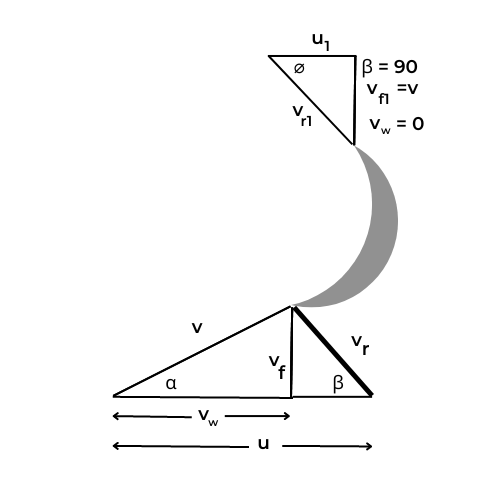
\includegraphics[width=0.97\linewidth]{img/velo_dia_prb.png}
  \caption{Velocity diagram}
\end{figure}

\begin{align*}
  u = \frac{\pi D N}{60} = \frac{\pi \times 0.6 \times 300}{60} = 9.42 \, m/s 
\end{align*}
\begin{align*}
  u_1 = \frac{\pi D_1 N}{60} = \frac{\pi \times 0.3 \times 300}{60} = 4.71 \, m/s 
\end{align*}

\begin{align*}
  V = \frac{V_f}{\sin \alpha} = \frac{3}{\sin 22} = 8.01 \, m/s 
\end{align*}
\begin{align*}
  V_w = V \cos \alpha = 8.01 \times \cos 22 = 7.42 \, m/s 
\end{align*}
Here, $u>v_w$

\begin{align*}
  \tan \theta &= \frac{V_f}{u-V_w} = \frac{3}{9.42-7.42}\\
  \Rightarrow \theta &= 56.4
\end{align*}

\begin{align*}
  \tan \phi &= \frac{V_{f_1}}{u_1} = \frac{3}{4.71} \\
  \Rightarrow \phi &= 32.5
\end{align*}
Here, $V_{f1} = v$ and $V_{w1}=0$

\begin{align*}
  Q &= \pi D B V_f = \pi \times 0.6 \times 0.15 \times 3 = 0.85 \, m^3/s
\end{align*}

\begin{align*}
  hp &= \frac{\rho Q V_w u}{746} \\
  &= \frac{1000 \times 0.85 \times 7.42 \times 9.42}{746}\\
  &= 79.65 \, hp
\end{align*}

\end{multicols}

\section{Lecture 11: Propeller Turbine}
\hfill Date: 24/07/2023

\begin{multicols}{2}  
  \subsection*{Problem-01}
  In an inward flow reaction turbine the inlet and outlet diameters are 3m and 2m respectively. The discharge through the turbine is 80 $m^3/s$ and the inlet vane angle is 120°. The discharge is radial at outlet and the velocity of flow at outlet is 13.6 m/s. The head of water is 162 m and width od the wheel is constant throughout. If the hydraulic efficiency is 88\%, Find the power produced and the speed of the turbine.

  \subsection*{Solution:}
  Given,
  \begin{align*}
    & D = 3 \, m \\
    & D_1 = 2 \, m \\
    & Q = 80 \, m^3/s \\
    & \theta = 120° \\
    & V_{f1} = 13.6 \, m/s \\
    & H = 162 \, m \\
    & \eta_h = 0.88
  \end{align*}

  Neglecting vane thickness factor,
  Q = $\pi D_1 B_1 V_{f1}$ \\
  \begin{align*}
    & 80 = \pi \times 2 \times B_1 \times 13.6 \\
    & B_1 = 0.94 \, m
  \end{align*}
  Here, $B = B_1$\\
  Again,
  \begin{align*}
    Q &= \pi D B V_f \\
    80 &= \pi \times 3 \times 0.94 \times V_f \\
    V_f &= 9.03 \, m/s
  \end{align*}

  Now, 
  \begin{align*}
    \tan (180-120) &= \frac{V_f}{u-V_{w}} \\
    \Rightarrow v_w &= u - 5.21 
  \end{align*}

  \begin{align*}
    \eta_h &= \frac{v_w u}{gH} \\
    0.88 &= \frac{u(u-5.21)}{9.81 \times 162} \\
    u &= 40.09 \, m/s
  \end{align*}

  \begin{align}
    u &= \frac{\pi D N}{60} \\
    N &= 255.22 \, rpm
  \end{align}
  
  so, $v_w$ = u - 5.21 = 34.88 m/s \\
  and, 
  \begin{align*}
    P_{out} &= \rho Q v_w  u \\
    &= 1000 \times 80 \times 34.88 \times 40.09 \\
    &= 111.867 \, MW
  \end{align*}
\end{multicols}
\pagebreak
\subsection*{Propeller Turbine}
\begin{multicols}{2}
  The propeller turbine is an axial flow turbine having a small number of blades usually 3 to 8. The runner is generally kept horizontal. That is the shaft is vertical.
  
  The following deviations from Francis Turbine should be carefully noted:\\

  \begin{enumerate}
    \item In case of propeller turbine the ratio 'n' is taken as - $$n = \frac{D_1}{D}$$ Where, $D_1$ = diameter of boss or hub on which the blades are mounted. And $D$ is the outside diameter of the runner.
    Now, Discharge, 
    \begin{align*}
      Q &= \frac{\pi}{4} \times (D^2 - D_1^2) \times V_f \\
      &= \frac{\pi}{4} \times (D^2 - D_1^2) \times \times \Psi \sqrt{2gH} \\
      &= \frac{\pi}{4} \times D^2 \times ( 1 - n^2) \times \Psi \sqrt{2gH} \\
    \end{align*} 
    The values of n ranges from 0.35 to 0.6. The value of $\Psi$ is about 0.7. 

    \item The peripheral velocity of u of the runner vanes depends upon the radius of the point under consideration. The blade angle varies from the rim of the boss and the vanes are warped. 
    \item The velocity triangle can be constructed at any radius. The expressions for work done is same as Francis turbine. 
    $$P = m v_w u $$

    \item The velocity of flow remains constant throughout.
  \end{enumerate}

\end{multicols}
  
\end{document}
